\documentclass[12pt,utf8,notheorems,compress,t]{beamer}
\usepackage{etex}

\usepackage[english]{babel}

\usepackage{mathtools}
\usepackage{booktabs}
\usepackage{array}
\usepackage{ragged2e}
\usepackage{multicol}
\usepackage{tabto}
\usepackage{xstring}
\usepackage{mathtools}
\usepackage{soul}\setul{0.2ex}{}
\usepackage[all]{xy}
\xyoption{rotate}
\usepackage{tikz}
\usetikzlibrary{calc,shapes.callouts,shapes.arrows}

\usepackage[protrusion=true,expansion=true]{microtype}

\newcommand{\A}{\mathcal{A}}
\newcommand{\E}{\mathcal{E}}
\newcommand{\F}{\mathcal{F}}
\renewcommand{\G}{\mathcal{G}}
\renewcommand{\O}{\mathcal{O}}
\newcommand{\K}{\mathcal{K}}
\newcommand{\ppp}{\mathfrak{p}}
\newcommand{\fff}{\mathfrak{f}}
\newcommand{\defeq}{\vcentcolon=}
\newcommand{\defeqv}{\vcentcolon\equiv}
\newcommand{\Sh}{\mathrm{Sh}}
\newcommand{\Set}{\mathrm{Set}}
\newcommand{\Sch}{\mathrm{Sch}}
\newcommand{\Hom}{\mathrm{Hom}}
\DeclareMathOperator{\Spec}{Spec}
\newcommand{\RelSpec}{\operatorname{\text{\ul{$\mathrm{Spec}$}}}}
\renewcommand{\_}{\mathpunct{.}}
\newcommand{\?}{\,{:}\,}
\newcommand{\speak}[1]{\ulcorner\text{\textnormal{#1}}\urcorner}

\setlength\parskip{\medskipamount}
\setlength\parindent{0pt}

\title{Using the internal language of toposes in algebraic geometry}
\author{Ingo Blechschmidt}
\date{November 27th, 2015}

\usetheme{Warsaw}
\usecolortheme{seahorse}
%\usefonttheme{default}?
%\usepackage{kurier}?
\usefonttheme{serif}
%\usepackage{libertine}?
\usepackage{mathpazo}
\useinnertheme{rectangles}

\setbeamertemplate{blocks}[rounded][shadow=false]

\newenvironment{changemargin}[2]{%
  \begin{list}{}{%
    \setlength{\topsep}{0pt}%
    \setlength{\leftmargin}{#1}%
    \setlength{\rightmargin}{#2}%
    \setlength{\listparindent}{\parindent}%
    \setlength{\itemindent}{\parindent}%
    \setlength{\parsep}{\parskip}%
  }%
  \item[]}{\end{list}}

\newcommand{\pointthis}[2]{%
  \tikz[remember picture,baseline]{\node[anchor=base,inner sep=0,outer sep=0]%
    (#1) {#1};\node[overlay,rectangle callout,%
    callout relative pointer={(-0.2cm,0.8cm)},fill=blue!20] at ($(#1.north)+(1.8cm,-1.4cm)$) {#2};}%
}%

\newcommand{\hcancel}[5]{%
  \tikz[baseline=(tocancel.base)]{
    \node[inner sep=0pt,outer sep=0pt] (tocancel) {#1};
    \draw[red, line width=0.4mm] ($(tocancel.south west)+(#2,#3)$) -- ($(tocancel.north east)+(#4,#5)$);
  }%
}

\newcommand{\slogan}[1]{%
  \begin{center}%
    \setlength{\fboxrule}{0pt}%
    \setlength{\fboxsep}{-14pt}%
    {\usebeamercolor[fg]{item}\fbox{\usebeamercolor[fg]{normal
    text}\parbox{0.9\textwidth}{\begin{center}#1\end{center}}}}%
  \end{center}%
}

\setbeamertemplate{frametitle}[default][colsep=-2bp,rounded=false,shadow=false,center]

\setbeamertemplate{headline}{}
\setbeamertemplate{navigation symbols}{}

\newcounter{framenumberpreappendix}
\newcommand{\backupstart}{
  \setcounter{framenumberpreappendix}{\value{framenumber}}
}
\newcommand{\backupend}{
  \addtocounter{framenumberpreappendix}{-\value{framenumber}}
  \addtocounter{framenumber}{\value{framenumberpreappendix}} 
}

\setbeamertemplate{footline}{%
  \begin{beamercolorbox}[wd=\paperwidth,ht=2.5ex,dp=1.25ex,right,rightskip=1mm,leftskip=1mm]{frametitle right}
    {\quad} \inserttitle \hfill \insertauthor \quad
    \insertframenumber\,/\,\inserttotalframenumber {\quad}
  \end{beamercolorbox}}

\newcommand{\hil}[1]{{\usebeamercolor[fg]{item}{\textbf{#1}}}}

\IfSubStr{\jobname}{\detokenize{nonotes}}{
  \setbeameroption{hide notes}
}{
  \setbeameroption{show notes}
}
\setbeamertemplate{note page}[plain]

\begin{document}

\begin{frame}[c]
  \centering
  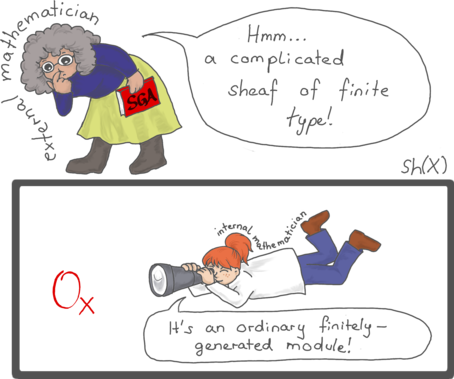
\includegraphics[scale=0.3]{images/external-internal-small}
  \medskip

  \hil{Using the internal language of toposes in \\ algebraic geometry}
  \medskip

  \scriptsize
  Ingo Blechschmidt \\
  University of Augsburg
  \medskip

  Topos à l'IHES \\
  November 27th, 2015
  \par
\end{frame}

\backupstart
\frame[t]{\frametitle{Outline}\scriptsize\begin{itemize}\item[]\tableofcontents\end{itemize}}

\begin{frame}[plain,c]
  \centering
  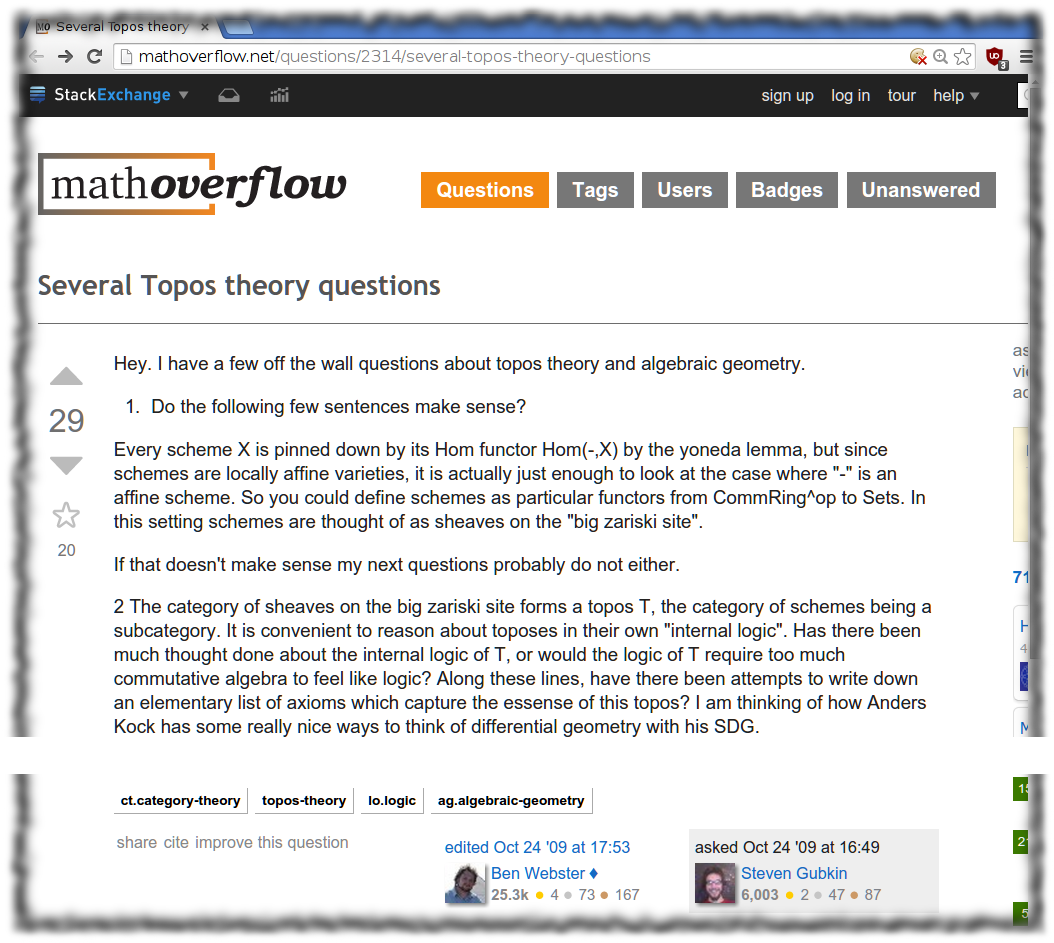
\includegraphics[scale=0.37]{images/math-overflow-steven-gubkin}
  \par
\end{frame}
\backupend


\section{Basic applications of the internal language}

\begin{frame}\frametitle{Exploiting the internal language}
  A \hil{scheme} is a locally ringed space~$(X,\O_X)$ which is
  locally isomorphic to the \hil{spectrum of a commutative ring}:
  \[ \Spec A \defeq \{ \ppp \subseteq A \,|\, \text{$\ppp$ is a prime ideal} \} \]
  \pause
  The topos~$\Sh(X)$ is the \hil{petit Zariski topos} of~$X$.

  \begin{center}
    \small
    \begin{tabular}{ll}
      \toprule
      externally & internally to $\Sh(X)$ \\
      \midrule
      sheaf of sets & set/type \\
      morphism of sheaves & map of sets \\
      monomorphism & injective map \\
      epimorphism & surjective map \\
      sheaf of rings & ring \\
      sheaf of modules & module \\
      \bottomrule
    \end{tabular}
  \end{center}
\end{frame}

\begin{frame}\frametitle{Building a dictionary}
  \slogan{\hil{Understand notions of algebraic geometry
  as notions of algebra internal to~$\boldsymbol{\Sh(X)}$.}}
  \begin{center}
    \small
    \scalebox{0.93}{\begin{tabular}{ll}
      \toprule
      externally & internally to $\Sh(X)$ \\
      \midrule
      sheaf of sets & set/type \\
      morphism of sheaves & map of sets \\
      monomorphism & injective map \\
      epimorphism & surjective map \\
      \midrule
      sheaf of rings & ring \\
      sheaf of modules & module \\
      sheaf of finite type & finitely generated module \\
      finite locally free sheaf & finite free module \\
      coherent sheaf & coherent module \\
      tensor product of sheaves & tensor product of modules \\
      rank function & minimal number of generators \\
      sheaf of rational functions & total quotient ring of~$\O_X$ \\
      \bottomrule
    \end{tabular}}
  \end{center}

  \visible<2>{\begin{tikzpicture}[overlay]
    \draw[fill=white, draw=white, opacity=0.9] (0,0) rectangle (\paperwidth,7.1);
    \node[anchor=south west,inner sep=0] (image) at (1.8,1.3) {
      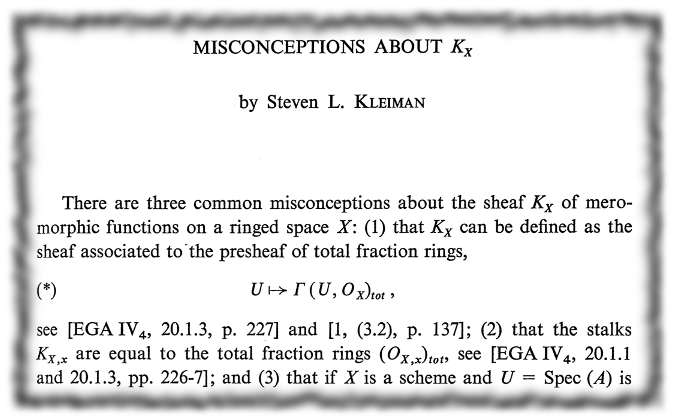
\includegraphics[width=0.7\textwidth]{images/steven-kleiman-misconceptions-about-kx}
    };
  \end{tikzpicture}}
\end{frame}

\begin{frame}[c]\frametitle{Praise for Mike Shulman}
  \centering
  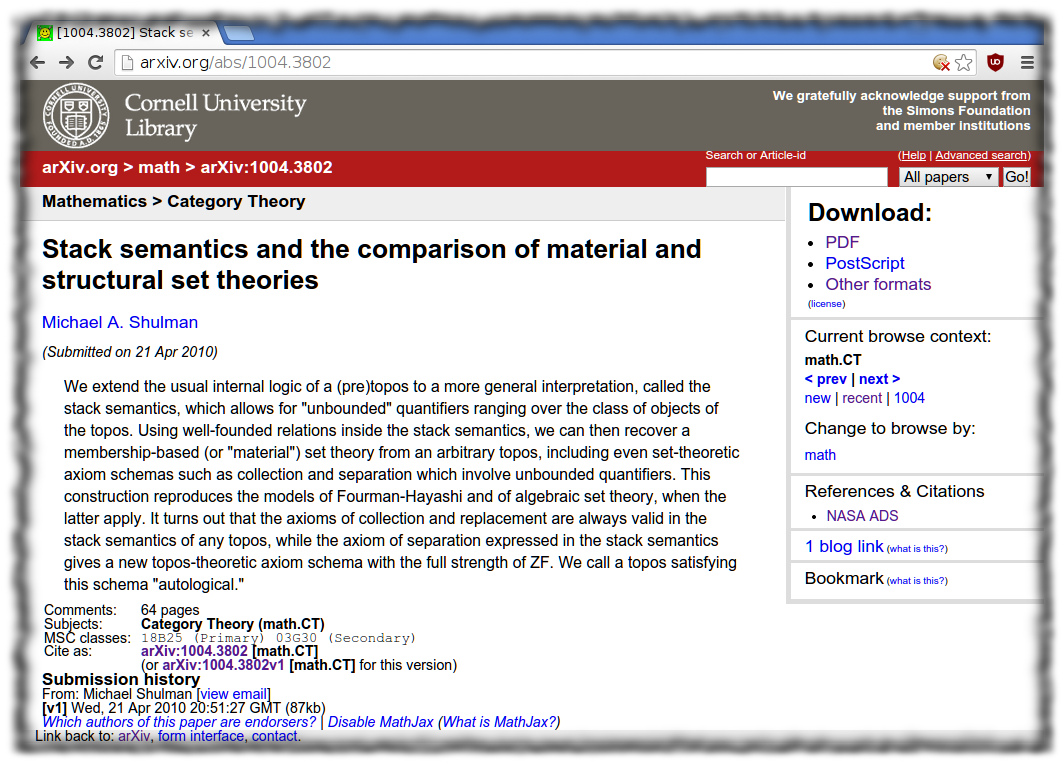
\includegraphics[scale=0.4]{images/mike-shulman-stack-semantics}
  \par
\end{frame}

\begin{frame}\frametitle{Using the dictionary}
  \begin{center}
    \begin{minipage}{0.75\textwidth}
      \begin{exampleblock}{}
        \justifying
        Let~$0 \to M' \to M \to M'' \to 0$ be a short exact sequence of
        modules. If~$M'$ and~$M''$ are finitely generated, so is~$M$.
      \end{exampleblock}
    \end{minipage}
    \medskip

    \scalebox{3}{$\Downarrow$}

    \begin{minipage}{0.75\textwidth}
      \begin{exampleblock}{}
        \justifying
        Let $0 \to \F' \to \F \to \F'' \to 0$ be a short exact sequence
        of~$\O_X$-modules. If~$\F'$ and~$\F''$ are of finite type, so
        is~$\F$.
      \end{exampleblock}
    \end{minipage}
  \end{center}
\end{frame}

\begin{frame}[c]\frametitle{Using the dictionary}
  \begin{center}
    \begin{minipage}{0.70\textwidth}
      \begin{exampleblock}{}
        \justifying
        Any finitely generated vector space does \emph{not not} possess a basis.
      \end{exampleblock}
    \end{minipage}
    \medskip

    \scalebox{3}{$\Downarrow$}

    \begin{minipage}{0.70\textwidth}
      \begin{exampleblock}{}
        \justifying
        Any sheaf of modules of finite type on a reduced scheme is locally free
        \emph{on a dense open subset}.
      \end{exampleblock}
      \centering
      \tiny Ravi Vakil: ``Important hard exercise'' (13.7.K).
      \par
    \end{minipage}
  \end{center}
\end{frame}

\begin{frame}\frametitle{A curious property}
  Let~$X$ be a scheme. Internally to~$\Sh(X)$,
  \begin{center}
    \hil{any non-invertible element of~$\boldsymbol{\O_X}$ is nilpotent.}
  \end{center}

  \centering
  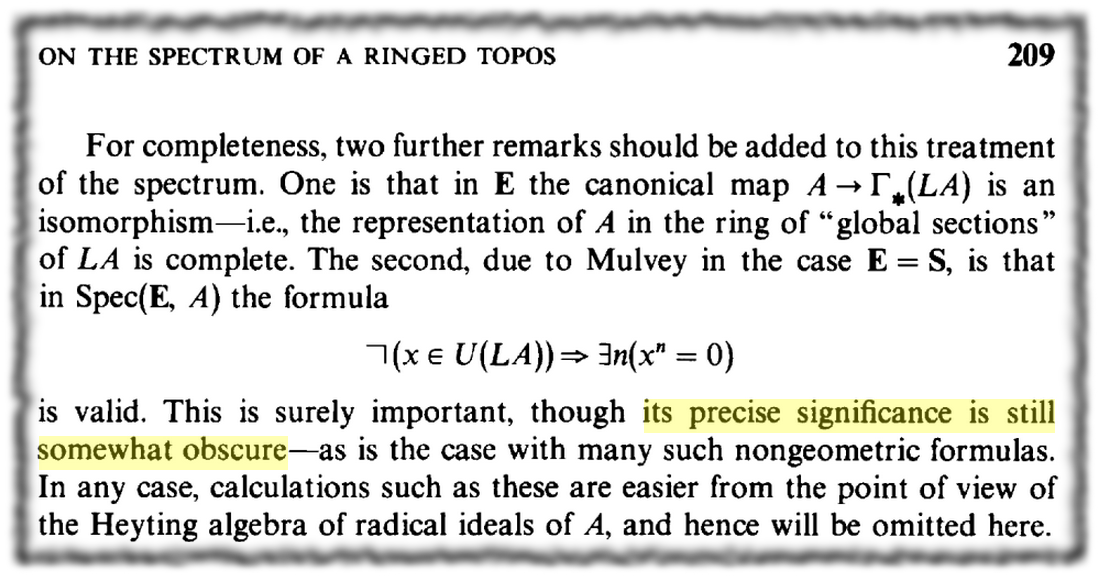
\includegraphics[scale=0.3]{images/tierney-on-the-spectrum-of-a-ringed-topos} \\
  \tiny
  %Miles Tierney. ``On the spectrum of a ringed topos''. \\ In: \emph{Algebra,
  %Topology, and Category Theory. A Collection of Papers in Honor of Samuel
  %Eilenberg}. Ed.\@ by A.~Heller and M.~Tierney. Academic Press, 1976,
  %pp.~189--210.
  Miles Tierney. On the spectrum of a ringed topos. 1976.
  \par
\end{frame}


\section{\texorpdfstring{The $\Diamond$-translation}{The ♢-translation}}

\newcommand{\idiamond}{{\usebeamercolor[fg]{item}{\boldsymbol{\Diamond}}}}
\newcommand{\gdiamond}[1]{\textcolor{gray}{\boldsymbol{\Diamond}(}#1\textcolor{gray}{)}}

\begin{frame}\frametitle{The $\Diamond$-translation}
  Let~$\E_\Diamond \hookrightarrow \E$ be a subtopos given by a \pointthis{local
  operator}{$\Diamond : \Omega_\E \to \Omega_\E$}~$\Diamond$. Then
  \[ \E_\Diamond \models \varphi \qquad\text{iff}\qquad
    \E \models \varphi^\Diamond\only<2->{.}\only<1>{,}\]
  \only<1>{where the translation~$\varphi \mapsto \varphi^\Diamond$ is given by:
  \begin{align*}
    (s = t)^\Diamond &\defeqv \idiamond(s=t) \\
    (\varphi \wedge \psi)^\Diamond &\defeqv \gdiamond{\varphi^\Diamond \wedge \psi^\Diamond} \\
    (\varphi \vee \psi)^\Diamond &\defeqv \idiamond(\varphi^\Diamond \vee \psi^\Diamond) \\
    (\varphi \Rightarrow \psi)^\Diamond &\defeqv \gdiamond{\varphi^\Diamond \Rightarrow \psi^\Diamond} \\
    (\forall x\?X\_ \varphi(x))^\Diamond &\defeqv \gdiamond{\forall x\?X\_ \varphi^\Diamond(x)} \\
    (\exists x\?X\_ \varphi(x))^\Diamond &\defeqv \idiamond(\exists x\?X\_ \varphi^\Diamond(x))
  \end{align*}}

  \only<2->{
    Let~$X$ be a scheme. Depending on~$\Diamond$,~$\Sh(X)
    \models \Diamond\varphi$ means that~$\varphi$ holds on \ldots
    \begin{itemize}
      \item \ldots{} a dense open subset.
      \item \ldots{} a schematically dense open subset.
      \item \ldots{} a given open subset~$U$.
      \item \ldots{} an open subset containing a given closed subset~$A$.
      \item \ldots{} an open neighbourhood of a given point~$x \in X$.
    \end{itemize}

    \pause
    Can tackle the question~``$\varphi^\Diamond \stackrel{?}{\Rightarrow} \Diamond\varphi$'' logically.
  }
\end{frame}


\section{Quasicoherence of sheaves of modules}

\begin{frame}\frametitle{Quasicoherence}
  Let~$X$ be a scheme. Let~$\E$ be an~$\O_X$-module.

  Then~$\E$ is quasicoherent
  if and only if, internally to~$\Sh(X)$,
  \begin{quote}\textnormal{$\E[f^{-1}]$ is a $\Diamond_f$-sheaf for any~$f : \O_X$, \\[0.3em]
  \qquad\qquad where~$\Diamond_f\varphi \defeqv (\text{$f$ invertible} \Rightarrow \varphi)$.}
  \end{quote}
  \pause

  In particular: If~$\E$ is quasicoherent, then internally
  \[ (\text{$f$ invertible} \Rightarrow s = 0) \Longrightarrow
    \bigvee_{n \geq 0} f^n s = 0 \]
  \vspace*{-1.5em}\par%
  for any~$f : \O_X$ and~$s : \E$.
\end{frame}


\section{The relative and internal spectrum}

\begin{frame}\frametitle{The absolute spectrum}
  Let~$A$ be a commutative ring (in~$\Set$).

  Is there a \hil{free local ring}~$A \to A'$ over~$A$?
  \[ \xymatrix{
    A \ar[rd] \ar[rrr] &&& R \\
    & A' \ar@{-->}[rru]
  } \]

  \hil{No,} if we restrict to~$\Set$.

  \hil{Yes,} if we allow a change of topos:
  Then $A \to \O_{\Spec A}$ is the universal localization.
\end{frame}

\newcommand{\defspeca}{\text{topological space of the prime ideals of $A$}}
\newcommand{\defspecb}{\text{topological space of the prime filters of $A$}}
\newcommand{\defspecc}{\text{locale of the prime filters of $A$}}

\begin{frame}\frametitle{The absolute spectrum, internalized}
  Let~$A$ be a commutative ring in a topos~$\E$.

  To construct the \hil{free local ring} over~$A$, give a constructive account
  of the spectrum:
  \begin{align*}
    \only<1>{\Spec A &\defeq \defspeca}
    \only<2->{\Spec A &\defeq \hcancel{$\defspeca$}{0pt}{3pt}{0pt}{-2pt}}
    \\
    \only<3>{&\defeq \defspecb}
    \only<4->{&\defeq \hcancel{$\defspecb$}{0pt}{3pt}{0pt}{-2pt}}
    \\
    \only<5->{&\defeq \defspecc}
  \end{align*}
  \pause
  \pause
  \pause
  \pause
  Define the frame of opens of~$\Spec A$ to be the frame of radical ideals
  in~$A$.
  \pause

  This gives an internal description of
  Monique Hakim's spectrum functor~$\mathrm{RT} \to \mathrm{LRT}$.
\end{frame}

\begin{frame}\frametitle{The relative spectrum}
  Let~$X$ be a scheme and~$\O_X \xrightarrow{\varphi} \A$ be a quasicoherent algebra.
  Can we describe~\hil{$\boldsymbol{\RelSpec_X \A}$}, a scheme over~$X$, internally?

  Desired universal property:
  \[ \Hom_{\Sch/X}(T, \RelSpec_X \A) \cong \Hom_{\mathrm{Alg}(\O_X)}(\A,
  \mu_*\O_T) \]
  for all~$X$-schemes~$T \xrightarrow{\mu} X$.
  \pause

  \hil{Solution:} Define internally the frame of~$\RelSpec_X \A$ to be the frame of
  those radical ideals~$I \subseteq \A$ such that
  \[ \forall f\?\O_X\_ \forall s\?\A\_
    (\text{$f$ invertible in~$\O_X$} \Rightarrow s \in I) \Longrightarrow
      fs \in I. \]
  \pause
  Its \hil{points} are those prime filters~$G$ of~$\A$ such that
  \[ \forall f\?\O_X\_ \varphi(f) \in G \Rightarrow \text{$f$ invertible in~$\O_X$}. \]
\end{frame}

\begin{frame}\frametitle{The relative spectrum, reformulated}
  Let~$B \to A$ be an algebra in topos.

  Is there a \hil{free local and local-over-$\boldsymbol{B}$ ring}~$A \to A'$ over~$A$?

  \[ \xymatrix{
    B \ar[r]\ar@/^2pc/[rrrr]^{\text{local}}\ar@/_/[rrd]_[@!-33]{\text{local}} &
      A \ar[rd] \ar[rrr] &&&
      {\substack{\text{local}\\\text{\normalsize$R$}\\\phantom{\text{local}}}} \\
    && {\substack{\text{\normalsize$A'$}\\\text{local}}} \ar@{-->}[rru]_[@!35]{\text{local}}
  } \]

  \medskip
  Form limits in the category of \hil{locally ringed locales}
  by \hil{relocalizing} the corresponding limit in ringed locales.
\end{frame}

\backupstart

\begin{frame}
  \slogan{\hil{Understand notions and statements of algebraic geometry
  as notions and statements of algebra internal to appropriate toposes.}}

  {\vspace{-0.5em}\centering
  \rotatebox{90}{\tiny\scalebox{0.5}{Illustration: Carina Willbold}}\hspace{-0.05cm}%
  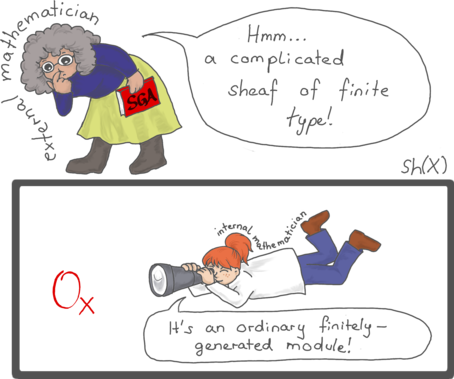
\includegraphics[scale=0.23]{images/external-internal-small}
  \par\medskip}

  \begin{itemize}
    \item Simplify proofs.
    \item Gain conceptual understanding.
    \item Develop a synthetic account of scheme theory.
  \end{itemize}

  \centering
  \hil{\href{http://tiny.cc/topos-notes}{http://tiny.cc/topos-notes}} \\
  \begin{minipage}{1.0\textwidth}\justifying
    \scriptsize
    spreading of properties,
    general transfer principles,
    applications to constructive algebra,
    quasicoherence,
    internal Cartier divisors,
    pullback along immersions $=$ internal sheafification,
    scheme dimension $=$ internal Krull dimension of~$\O_X$,
    dense $=$ not not,
    modal operators,
    relative spectrum,
    other toposes,
    étale topology,
    group schemes $=$ groups,
    \ldots
  \end{minipage}
  \par
\end{frame}
% Fun fact:
% Very naive definition of P^n works internal to the big Zariski topos.

\begin{frame}[plain,c]
  \centering
  
\includegraphics[scale=0.5]{images/sheafification-man}
  \sffamily

  You should totally look up:

  \hil{The Adventures of Sheafification Man}
  \par
\end{frame}

\begin{frame}\frametitle{Spreading from points to neighbourhoods}
  All of the following lemmas have a short, sometimes trivial proof.
  Let~$\F$ be a sheaf of finite type on a ringed space~$X$.
  Let~$x \in X$. Let~$A \subseteq X$ be a closed subset. Then:
  \small
  \begin{itemize}
    \item $\F_x = 0$ iff~$\F|_U = 0$ for some open neighbourhood of~$x$.
    \item $\F|_A = 0$ iff~$\F|_U = 0$ for some open set containing~$A$.
    \item $\F_x$ can be generated by~$n$ elements iff this is true on some open
    neighbourhood of~$x$.
%   \item $\alpha_x$ is surjective iff~$\alpha$ is an epimorphism on some open
%   set containing~$x$, where~$\alpha : \G \to \F$ is any morphism.
    \item $\mathcal{H}\mathrm{om}_{\O_X}(\F,\G)_x \cong
    \Hom_{\O_{X,x}}(\F_x,\G_x)$ if~$\F$ is of finite presentation around~$x$.
    \item $\F$ is torsion iff~$\F_\xi$ vanishes (assume~$X$ integral and~$\F$ quasicoherent).
    \item $\F$ is torsion iff~$\F|_{\mathrm{Ass}(\O_X)}$ vanishes (assume~$X$
    locally Noetherian and~$\F$ quasicoherent).
  \end{itemize}
\end{frame}

\begin{frame}\frametitle{The smallest dense sublocale}
  Let~$X$ be a reduced scheme satisfying a technical condition.
  Let~$i : X_{\neg\neg} \to X$ be the inclusion of the smallest dense sublocale
  of~$X$.

  Then~$i_* i^{-1} \O_X \cong \K_X$.

%  \begin{itemize}
%    \item This is a highbrow way of saying ``rational functions are regular
%    functions which are defined on a dense open subset''.
%    \item There is a generalization to nonreduced schemes.
%  \end{itemize}
\end{frame}

\begin{frame}\frametitle{Transfer principles}
  Let~$M$ be an~$A$-module. How do~$M$ and the sheaf~$M^{\sim}$ on~$\Spec A$
  relate?

  Observe that $M^{\sim} \cong \underline{M}[F^{-1}]$ is the localization of~$M$ at
  the \hil{generic filter}. Therefore:
  \begin{center}
    $M^{\sim}$ inherits all those properties of~$M$ which are \\
    \hil{stable under localization}.
  \end{center}
  Examples: finitely generated, free, flat, \ldots

  A converse holds as well, suitably formulated.
\end{frame}

\begin{frame}\frametitle{The gros Zariski topos}
  Let~$X$ be a scheme. The \hil{gros Zariski topos} is the topos of sheaves
  on~$\Sch/X$ with respect to the Zariski topology. From its point of view,
  \ldots

  \begin{itemize}
    \item \ldots{} $X$-schemes look just like sets,
    \item \ldots{} $\mathbb{P}^n_X$ is given by the naive expression
    \[ \{ (x_0,\ldots,x_n) \,|\, x_1 \neq 0 \vee \cdots \vee x_n \neq 0
    \}/\text{(rescaling)}, \]
    \item \ldots{} affinity is a ``double dual condition'', and
    \item \ldots{} the étale topology is the coarsest topology~$\Diamond$ s.\,th.
    \[ \forall f : \mathbb{A}^1_X[T]\_\
      \text{$f$ is monic separable} \Rightarrow
      \Diamond(\exists t : \mathbb{A}^1\_ f(t) = 0). \]
  \end{itemize}
\end{frame}

\begin{frame}\frametitle{Translating internal statements}
  Let~$X$ be a topological space (or locale) and let~$\alpha : \F \to \G$ be a
  morphism of sheaves on~$X$. Then:
  \allowdisplaybreaks
  \begin{align*}
    & \Sh(X) \models \speak{$\alpha$ is injective} \\[0.5em]
    \Longleftrightarrow\
    & \Sh(X) \models \forall s\?\F\_ \forall t\?\F\_ \alpha(s) = \alpha(t) \Rightarrow s = t \\[0.5em]
    \Longleftrightarrow\ &
      \text{for all open~$U \subseteq X$, sections $s \in \F(U)$:} \\
    &\qquad
      \text{for all open~$V \subseteq U$, sections $t \in \F(V)$:} \\
    &\qquad\qquad
        \text{for all open~$W \subseteq V$:} \\
    &\qquad\qquad\qquad
          \text{$\alpha_W(s|_W) = \alpha_W(t|_W)$ implies $s|_W = t|_W$} \\[0.5em]
    \Longleftrightarrow\ &
      \text{for all open~$U \subseteq X$, sections $s, t \in \F(U)$:} \\
    &\qquad
          \text{$\alpha_U(s|_U) = \alpha_U(t|_U)$ implies $s|_U = t|_U$} \\[0.5em]
    \Longleftrightarrow\ &
      \text{$\alpha$ is a monomorphism of sheaves}
  \end{align*}
\end{frame}

\backupend

\end{document}

1. Tell story; begin with MO question
2. Basics (include praise for Mike Shulman)
3. Curious field property and more advanced examples
4. Relative spectrum (also mention equivalence to Hakim's spectrum in dimension zero)
5. Outlook: synthetic algebraic geometry, relative geometry, big Zariski topos

\note{\justifying\fontsize{8pt}{9.6}\selectfont
  \begin{center}\large\textbf{Abstract}\end{center}

  \begin{changemargin}{2.5em}{2.5em}
    We describe how the internal language of certain
    toposes, the associated petit and gros Zariski toposes of a scheme, can be
    used to give simpler definitions and more conceptual proofs of the basic
    notions and observations in algebraic geometry.
    % This is useful for studying schemes from a local or relative point of view.

    The starting point is that, from the internal point of view, sheaves of rings
    and sheaves of modules look just like plain rings and plain modules.
    In this way, some concepts and statements of scheme theory can be reduced to
    concepts and statements of intuitionistic linear algebra.

    Furthermore, modal operators can be used to model phrases such as ``on a
    dense open subset it holds that'' or ``on an open neighbourhood of a given
    point it holds that''. These operators define certain subtoposes; a
    generalization of the double-negation translation is useful in order to
    understand the internal universe of those subtoposes from the internal point
    of view of the ambient topos.

    A particularly interesting task is to internalize the
    construction of the relative spectrum, which, given a quasicoherent sheaf of algebras
    on a scheme~$X$, yields a scheme over~$X$. From the internal point of
    view, this construction should simply reduce to an intuitionistically sensible
    variant of the ordinary construction of the spectrum of a ring, but it turns
    out that this expectation is too naive and that a refined approach is
    necessary.
  \end{changemargin}
}

  \scriptsize
  \begin{itemize}
    \item $\Sh(X) \models f = g$ iff~$f = g \in \F(X)$.
    \item $\Sh(X) \models f = g \vee f = h$ iff on a cover~$X = \bigcup_i U_i$,
    $f|_{U_i} = g|_{U_i}$ or~$f|_{U_i} = h|_{U_i}$.
    \item $\Sh(X) \models \neg\neg(f = g)$ iff~$f = g$ on a dense open subset
    of~$X$.
  \end{itemize}

\begin{frame}\frametitle{The internal language of a topos}
  Let~$\E$ be a topos. Then we can define the meaning of
  \[ \hil{$\E \models \varphi \qquad\textnormal{(``$\varphi$ holds in $\E$'')}$} \]
  for formulas~$\varphi$ over~$\E$ using the \hil{Kripke--Joyal semantics}.

  \begin{center}
    \small
    \begin{tabular}{ll}
      \toprule
      externally & internally \\
      \midrule
      object & set/type \\
      morphism & map of sets \\
      monomorphism & injective map \\
      epimorphism & surjective map \\
      \bottomrule
    \end{tabular}
  \end{center}
  \pause

  \mbox{If~$\varphi$ implies~$\psi$ \hil{intuitionistically}, then~$\E \models \varphi$
  implies~$\E \models \psi$.}
\end{frame}

\begin{frame}\frametitle{Limits of locally ringed locales}
  Let~$(X_i)_i$ be a diagram of locally ringed locales.

  Its limit is given by \hil{relocalizing} the corresponding limit
  in~$\mathrm{RL}$.
\end{frame}
% Mention only orally?
% Phrase more categorically.
% Extend to toposes.
